% $Header: /cvsroot/latex-beamer/latex-beamer/examples/beamerexample5.tex,v 1.22 2004/10/08 14:02:33 tantau Exp $

\docdntntcla[s[11p1]{bct[1rp
t]{beamer}

\usetheme{Darmstadt}

\usepackage{times}
\usefonttheme{structurebold}

%\usepackage[english]{babel}
\usepackage[portuges]{babel}
\usepackage{pgf,pgfarrows,pgfnodes,pgfautomata,pgfheaps}
\usepackage{amsmath,amssymb}
\usepackage[latin1]{inputenc}
\usepackage{graphicx}

\setbeamercovered{dynamic}

\newcommand{\Lang}[1]{\operatorname{\text{\textsc{#1}}}}

\newcommand{\Class}[1]{\operatorname{\mathchoice
  {\text{\sf \small #1}}
  {\text{\sf \small #1}}
  {\text{\sf #1}}
  {\text{\sf #1}}}}

\newcommand{\NumSAT}      {\text{\small\#SAT}}
\newcommand{\NumA}        {\#_{\!A}}

\newcommand{\barA}        {\,\bar{\!A}}

\newcommand{\Nat}{\mathbb{N}}
\newcommand{\Set}[1]{\{#1\}}

\pgfdeclaremask{tu}{beamer-tu-logo-mask}
\pgfdeclaremask{computer}{beamer-computer-mask}
\pgfdeclareimage[interpolate=true,mask=computer,height=2cm]{computerimage}{beamer-computer}
\pgfdeclareimage[interpolate=true,mask=computer,height=2cm]{computerworkingimage}{beamer-computerred}
\pgfdeclareimage[mask=tu,height=.5cm]{logo}{logounesp}

\logo{\pgfuseimage{logo}}

\title{Significado F�sico do Calor Espec�fico}
\author{Ney Lemke}
\institute[IBB-UNESP]{%
    Departamento de F�sica e Biof�sica}
\date{ 2011}                                

\colorlet{redshaded}{red!25!bg}
\colorlet{shaded}{black!25!bg}
\colorlet{shadedshaded}{black!10!bg}
\colorlet{blackshaded}{black!40!bg}

\colorlet{darkred}{red!80!black}
\colorlet{darkblue}{blue!80!black}
\colorlet{darkgreen}{green!80!black}

\def\radius{0.96cm}
\def\innerradius{0.85cm}

\def\softness{0.4}
\definecolor{softred}{rgb}{1,\softness,\softness}
\definecolor{softgreen}{rgb}{\softness,1,\softness}
\definecolor{softblue}{rgb}{\softness,\softness,1}

\definecolor{softrg}{rgb}{1,1,\softness}
\definecolor{softrb}{rgb}{1,\softness,1}
\definecolor{softgb}{rgb}{\softness,1,1}

\AtBeginSection[]{\frame{\frametitle{Outline}\tableofcontents[current]}}

\begin{document}

\frame{\titlepage}

%\section*{Outline}

\part{Parte I}

\frame{\frametitle{Outline} 
\tableofcontents[part=1]}
\section{Temperatura: Perspectiva Microsc�pica}
\frame{\frametitle{Defini��o de Temperatura}

Definimos a Temperatura de um sistema na termodin�mica:

$$\frac{1}{T}=\left( \frac{\partial S}{\partial U}\right)_{V,N}$$

Esta equa��o relaciona a temperatura ao aumento de entropia causado por um aumento de energia. 
}

\frame{\frametitle{Sistema de dois estados:}
\begin{center}
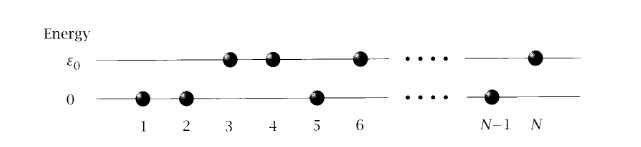
\includegraphics[scale=0.4]{doisestados}
\end{center}
}


\frame{\frametitle{Sistema de dois estados:}
      \begin{itemize}
      \item $n$ part�culas no estado excitado ($\epsilon_o>0$)
      \item $N-n$ part�culas no estado fundamental 
      \end{itemize}
}


\frame{\frametitle{Sistema de dois estados:}
Energia:

$$U=n\epsilon_o$$

$$W=\frac{N!}{n!(N-n)!}$$

$$\frac{S}{k}=\ln W=-n\ln \frac{n}{N}-(N-n)\ln \left(\frac{N-n}{N} \right)$$

$$\frac{1}{T}=k\left( \frac{\partial \ln W}{\partial U} \right)_{V,N}
=k\left( \frac{\partial \ln W}{\partial n} \right)_{V,N}
\left(\frac{dn}{du}  \right)$$
}

\frame{\frametitle{Sistema de dois estados:}
$$\frac{1}{T}=-\frac{k}{\epsilon_o}\ln \left(\frac{n/N}{1-n/N} \right)
%=-\frac{k}{\epsilon_o}\ln \left( \frac{U/N\epsilon}{1-U/N} \right)
$$


$$\frac{1}{T}=\frac{k}{\epsilon_o}\ln \left(\frac{f_{ground}}{f_{excited}} \right)$$

}



\frame{\frametitle{Sistema de dois estados:}
\begin{center}
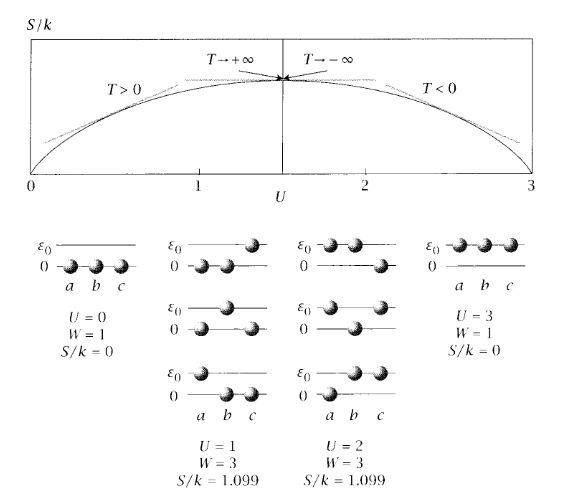
\includegraphics[scale=0.4]{temperatura}
\end{center}
}


\frame{\frametitle{Sistema de dois estados:}
  \begin{description}
  \item[$T>0$] Para sistemas com baixa energia a temperatura � positiva. Estes sistemas abosorvem energia para atingir o m�ximo da multiplicidade.
\item[$T=0$] Estes sistemas possuem metade dos �tomos em cada n�vel de energia. 

  \item[$T<0$] Sistemas com valores elevados de energia possuem temperatura negativa, ou seja esses sistemas devem perder energia para maximimizar sua multiplicidade. 

  \end{description}
}
\section{Calor Espec�fico}
\frame{\frametitle{Significado F�sico do Calor Espec�fico }

O calor espec�fico mede a quantidade de calor necess�ria 
para aumentar a temperatura de um corpo. Neste caso vamos considerar $C_V$ 
e um sistema em contato com um banho t�rmico. 

Devido ao contato com o banho a Temperatura do Corpo flutua aleatoriamente. 

}


\frame{\frametitle{Densidade de estados}

$$p(E)=\frac{W(E)e^{-\beta E}}{Q}$$

$W(E)$ � a denisdade de estados, ou seja o n�mero de estados com uma determinada
energia $E$.
 
\begin{center}
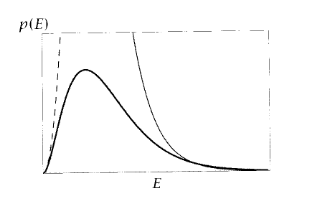
\includegraphics[scale=0.4]{densidadeestados}
\end{center}
}

\frame{\frametitle{Flutua��es}
Vamos avaliar esta quantidade na proximidade do m�ximo. Vamos assumir
que o banho t�rmico possui temperatura $T_o$ e que $\beta=1/kT_o$.

$$\ln p(E)=\ln p(U)+(E-U) (\ln p(U))^\prime +\frac{(E-U)^2}{2} (\ln p(U))^{\prime\prime}$$

Sabemos que no m�ximo $E=\langle E\rangle=U$. Como estamos no m�ximo:

$$(\ln p(U))^\prime=0$$


$$(\ln p(U))^{\prime\prime}=(\ln W -\beta)^{\prime\prime}=(S/k -\beta)^{\prime\prime}$$


}

\frame{\frametitle{Flutua��es}
$$(\ln p(U))^{\prime\prime}=(\ln W -\beta)^{\prime\prime}=(S/k -\beta)^{\prime\prime}$$

$$(\ln p(U))^{\prime\prime}=(S/k -\frac{1}{kT_o})^{\prime\prime}
=\left( \frac{1}{kT}\right)^\prime$$

$$=\frac{-1}{kT^2}\left( \frac{\partial T}{\partial E} \right)_{E=U}$$

$$=\frac{-1}{kT_o^2C_V}$$
}

\frame{\frametitle{Flutua��es}

$$p(E)=Ce^{\frac{-(E-U)^2}{2kT_o^2C_V}}$$

Como essa fun��o � gaussiana sabemos que:

$$\sigma^2=\langle (E-U)^2\rangle=kT_o^2C_V$$

Uma Quantidade interessante �

$$\frac{\sigma}{U}\sim \frac{\sqrt{N}}{N}\sim N^{-1/2}$$

Ou seja no limite termodin�mico as flutua��es s�o desprez�veis.
Para $N\sim 10^{23}$, as flutua��es seriam $10^{-11}$, inacess�veis experimentalmente.


}
\end{document}

